\begin{frame}{Rete elettrica attuale}
	\begin{figure}[h] 
		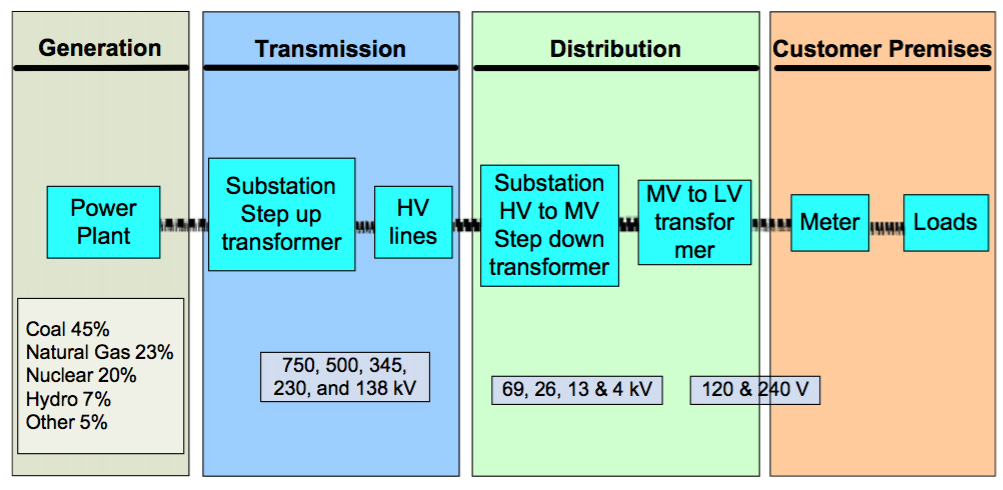
\includegraphics[scale=0.25, cfbox=blue_slides 1pt 0pt]{imgs/elect_grid.png}
		%\caption{Rete elettrica attuale}
	\end{figure}

\begin{itemize}[<+- | alert@+>]
	\item Tre sottosistemi distinti
		\begin{itemize}
		\item Generazione
		\item Trasmissione
		\item Distribuzione
		\end{itemize}
\end{itemize}
\end{frame}

\begin{frame}{Rete elettrica attuale}
	\begin{itemize}[<+- | alert@+>]
	\item Comunicazione unidirezionale
	\item Interconnessione e ridondanza per risolvere i problemi
	\item Distribuzione dell'energia gestita da un controllore centralizzato
	\end{itemize}

\end{frame}

\begin{frame}{Problemi della rete elettrica attuale}
	\begin{itemize}[<+- | alert@+>]
	\item Numerosi problemi da risolvere
		\begin{itemize}
		\item Diversificazione della generazione di energia
		\item Gestione delle richieste utente
		\item Conservazione dell’energia
		\item Riduzione globale dell’emissione di anidride carbonica
		\end{itemize}
	\item Non ci si può affidare all'infrastruttura attuale
		\begin{itemize}
			\item Inadeguatezza della struttura gerarchica
			 	\begin{itemize}
			 	\item Effetto domino in caso di guasti
			 	\end{itemize}
		\end{itemize}
	\end{itemize}
\end{frame}

\begin{frame}{Problemi della rete elettrica attuale}
	\begin{itemize}[<+- | alert@+>]
	\item Necessità di digitalizzare le infrastrutture critiche
		\begin{itemize}
		\item Aggiunta di capacità di computazione e comunicazione
		\item Requisito necessario per gestire l'ambiente che muta
		\end{itemize}
	\item Esempio di digitalizzazione: meter analogico $\rightarrow$ Smart meter
		\begin{itemize}
			\item Dispositivo disconnesso e non critico $\rightarrow$ Dispositivo connesso ad Internet che può generare dati critici
		\end{itemize}
\item Fondamentale la sicurezza dei dati e dei comandi degli smart meter
\item Obiettivo della survey: capire la sicurezza della nuova infrastruttura
	\end{itemize}
\end{frame}

\begin{frame}{Perché la Smart Grid?}
	\begin{itemize}[<+- | alert@+>]
	\item Vari fattori influenzano lo sviluppo della rete elettrica
	 \begin{itemize}
	  	\item Strutture non più adeguate
	  	\item Vincoli termici e operativi
	  	\item Sicurezza delle forniture
	  	\item Iniziative nazionali
	 \end{itemize}
	\item Significative opportunità offerte da 
	\begin{itemize}
	\item ICT
	\item Monitoraggio costante delle componenti della rete
	\end{itemize}
	\end{itemize}
\end{frame}


\begin{frame}{Perché la Smart Grid?}
	\begin{figure}[h] 
		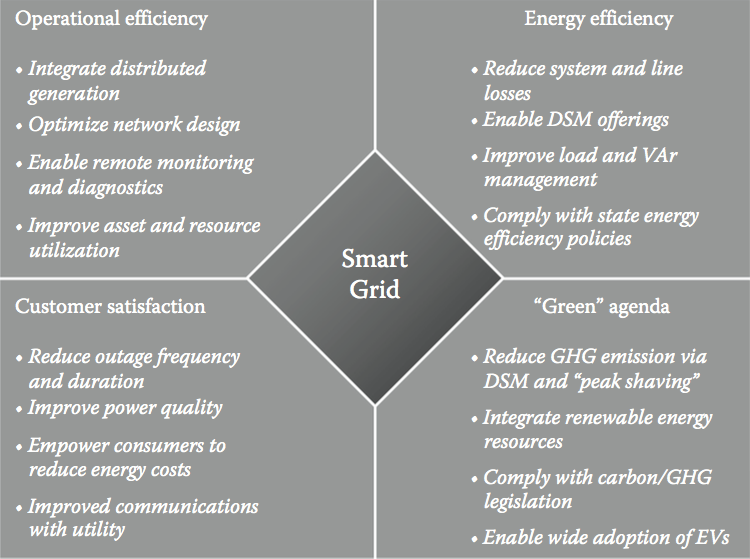
\includegraphics[scale=0.3, cfbox=blue_slides 1pt 0pt]{imgs/benefits.png}
		%\caption{Vantaggi introdotti dalla Smart Grid}
	\end{figure}
\end{frame}


\begin{frame}{Smart Grid: definizione}
\begin{itemize}[<+- | alert@+>]
\item Smart Grid = tecnologie + soluzioni per utenti finali
\item Non esiste una singola definizione precisa
\item È possibile trovare una serie di caratterizzazioni
\end{itemize}
\end{frame}

\begin{frame}{Smart Grid: definizione}
\begin{block}{Secondo l’European Technology Platform}
\begin{quote}
\textit{``Una Smart Grid è una rete elettrica che può integrare intelligentemente le azioni di tutti gli utenti connessi ad essa - generatori, consumatori - in modo da fornire efficientemente un’alimentazione elettrica che sia sostenibile, economica e sicura.”}
\end{quote}
\end{block}
\end{frame}

\begin{frame}{Smart Grid: definizione}
\begin{block}{In accordo all’US Department of Energy}
\begin{quote}
\textit{``Una Smart Grid utilizza la tecnologia digitale per migliorare l’affidabilità, la sicurezza e l’efficienza (sia economica che energetica) del sistema elettrico, a partire dalla generazione su larga scala, attraverso il sistema di distribuzione, fino ai consumatori, ed attraverso un numero crescente di risorse di storage e di generazione distribuita.”}
\end{quote}
\end{block}
\end{frame}


\begin{frame}{Smart Grid: definizione}
\begin{block}{Per \textit{Smarter Grids: The Opportunity}}
\begin{quote}
\textit{``Una Smart Grid utilizza sensing, embedded processing e comunicazioni digitali per far sì che la rete elettrica sia osservabile (capace di essere misurata e visualizzata), controllabile (capace di essere manipolata ed utilizzata), automatizzata (capace di adattarsi ed autoripararsi), pienamente integrata (pienamente interoperabile con sistemi esistenti e con la capcità di incorporare un insieme di diverse sorgenti energetiche).”}
\end{quote}
\end{block}
\end{frame}


\begin{frame}{Requisiti di una Smart Grid}
\begin{itemize}[<+- | alert@+>]
\item Quality of Service
	\begin{itemize}
		\item Bassa latenza: la maggior parte delle interazioni deve avvenire in tempo reale
		\item Larghezza di banda sufficiente per permettere la trasmissione simultanea di messaggi senza impatto sulla latenza
	\end{itemize}
\item Interoperabilità
	\begin{itemize}
		\item Abilità delle diverse parti della Smart Grid di lavorare insieme
	\end{itemize}
\end{itemize}
\end{frame}

\begin{frame}{Requisiti di una Smart Grid}
\begin{itemize}[<+- | alert@+>]
\item Scalabilità
	\begin{itemize}
		\item Facilitare l’inserimento di nuovi dispositivi, nuovi servizi, e meccanismi di monitoraggio real-time
	\end{itemize}
\item Standardizzazione
	\begin{itemize}
		\item IEEE P2030 group si occupa di definire standard e linee guida
	\end{itemize}
\end{itemize}
\end{frame}

\begin{frame}{Requisiti di una Smart Grid}
\begin{itemize}[<+- | alert@+>]
\item Sicurezza
	\begin{itemize}
		\item Gestire attacchi volontari (terrorismo, spionaggio, utenti non contenti)
		\item Gestire manomissioni involontarie (fallimenti delle attrezzature, disastri naturali)
		\item North American Electrical Reliability Corporation-Critical Infrastructure Protection (NERC-CIP), IEEE, National Infrastructure Protection Plan (NIPP), e NIST stabiliscono i requisiti di sicurezza della Smart Grid
		\item Denominatore comune: autenticazione, autorizzazione e tecnologie per la privacy
	\end{itemize}
\end{itemize}
\end{frame}


\begin{frame}{Building Blocks: requisiti}
\begin{itemize}[<+- | alert@+>]
\item Building blocks rete elettrica $\rightarrow$ Smart Grid
\begin{itemize}
	\item Monitoraggio/sensing
	\item Comunicazione
	\item Controllo
\end{itemize}
\item Requisiti
\begin{itemize}
\item Rilevare malfunzionamenti/deviazioni dal normale range operativo
\item Permettere che l’input dei sensori raggiunga gli elementi di controllo
\item Generare messaggi per assicurarsi che la trasmissione sia conforme alle aspettative
\end{itemize}
\end{itemize}
\end{frame}
